18. \begin{figure}[ht!]
\center{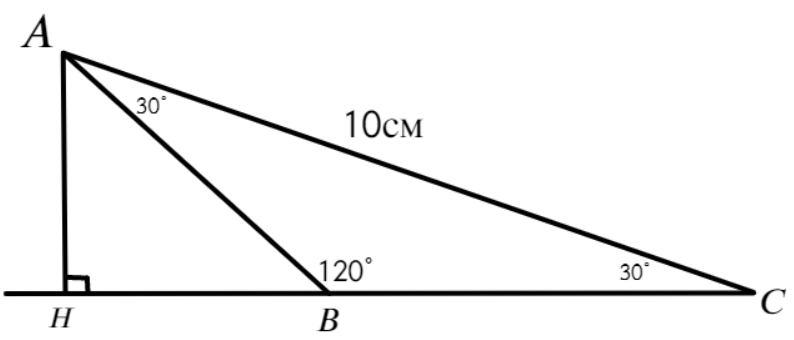
\includegraphics[scale=0.35]{g18.png}}
\end{figure}\\
Углом в $120^\circ$ может быть только угол при вершине, тогда углы при основании треугольника равны $(180^\circ-120^\circ):2=30^\circ.$ Поэтому в прямоугольном треугольнике $AHC$ катет $AH$ лежит напротив угла $30^\circ,$ а значит равен половине гипотенузы $AC.$ Таким образом, $AH=10:2=5$ см.\\
